\label{chapter:problems}

Writing Multithreaded programs can encounter concurrency errors and performance anomalies. This thesis discusses in detail two different types of problems, non-determinism and false sharing.  We discuss the definitions, causes of these problems and their possible consequence as follows.

\section{Non-determinism}
\label{sec:nondeterminism}

\subsection{Background}
Deterministic behavior of programs is the most desirable behavior: given the same input, a program
produces the same output and generates the same execution. Relying on this behavior, it is able to figure out problems of programs. 

In reality, it is relatively easy for sequential programs to achieve this target if a program do not explicitly rely on a randomized mechanism. 
However, it is hard to do this for parallel programs. In shared memory multithreaded programs, an application can only experience one of many possible 
schedules at a time. Thread scheduling, the order of memory accesses on the shared data, operations depending on timing and non-deterministic synchronizations, can easily lead to different executions of the same program.


\begin{figure*}[!ht]
{\centering
\fbox{
\subfigure{\lstinputlisting[numbers=none,frame=none,boxpos=t]{fig/nondeter.sample1}}
\hspace{20pt}
\subfigure{\lstinputlisting[numbers=none,frame=none,boxpos=t]{fig/nondeter.sample2}}
\hspace{20pt}
\subfigure{\lstinputlisting[numbers=none,frame=none,boxpos=t]{fig/nondeter.sample3}}
}
\caption{Non-determinism problem 
\label{fig:nondeterminism}}
}
\end{figure*}

A simple example of non-deterministic execution can be seen in Figure~\ref{fig:nondeterminism}. When using the standard \pthreads{} library, this program can print ``1,0'', ``0,1'' or ``1,1'' in the end, depending on the order of memory accesses from different threads. We actually run this simple program for one million times. About 99.43\% of time, it will print ``1,0'', while 0.56\% it will print ``0,1'' and 0.01\% it will print ``1,1''. According to the semantics of this program, both ``1,0'' and ``1,0'' are correct results. Thus, the unexpected result (``1,1'') caused by race conditions happens very rarely, only about 0.01\%.  
It is very difficult to observe/reproduce these rare cases that caused by race conditions.

\subsection{Source of Non-determinism}
Non-determinism can be caused by a lot of sources, both external sources and internal sources. For example, the timing of external inputs is one of the sources that can lead to non-determinism. This section only lists internal sources of non-determnism~\cite{costofdeterminism}. 
 
\emph{Thread Communication}: 
Thread communication is the most important source of non-determinism for multithreaded programs. 
First, the order of accesses on shared variables may change from one execution to the other. Second, the orders on shared resources, such as memory allocation, synchronization, and library/system calls, vary across different executions. 
Third, the interaction between compiler and run-time can be changed. For example, lazy binding may cause the thread that  performs address resolution to execute much more instructions than others. 

\emph{Memory Layout}: 
Address space layout randomization (ASLR) in Linux environment brings non-deterministic memory addresses of instructions and data across different executions. Thus, a program relying on memory addresses lead to non-deterministic execution of a program. 

\emph{System or Library Dependence}:
Some library or system calls cannot return deterministic results. For example, the \texttt{gettimeofday()} library call returns different time values at different time, and \texttt{read} system calls may return different number of bytes, depending on the timing of issuing \texttt{read} calls.  An application relying on them can execute non-deterministically too. 


\subsection{Effect of Non-determinism}
Because of different sources of non-determinism, listed in the above section, existing multithreaded applications can not run deterministically: given the same input, a program can have different executions that may or may not lead to different outputs. 

Non-determinism can greatly complicate the reasoning and debugging in development phases, which makes it hard for programmers to reproduce program errors. 
Even worse, since executions of deployment can vary from executions of development phase, a lot of programmer errors can be easily leaked to customers.

By contrast, determinism greatly simplifies the understanding and debugging of multithreaded programs. We can always guarantee the same executions on both development phases and the deployment phases, thus there is no need to worry about erroneous results. 

\section{False Sharing}
\label{sec:falsesharingproblems}

\subsection{Definition}
% What is the definition of false sharing?
False sharing occurs when different processors in a shared-memory parallel system are referencing distinct fields within the same coherence block (page or cache line) simultaneously, thereby inducing ``unnecessary'' coherence traffic~\cite{Bolosky:1993:FSE:1295480.1295483}. 

Although it is difficult or impossible to know where a thread runs in an actual execution, we can conservatively assume that different threads are running on different processors with separate cache. Thus, in the multithreaded environment, false sharing simply implies: multiple threads access distinct parts of the same cache line simultaneously, while one of them is a write operation. False sharing is shown in Figure~\ref{fig:fs}. 
Based on the relationship of false sharing objects, 
false sharing can be classified into inter-object and intra-object false sharing. When two different objects in the same cache line are accessed by different threads simultaneously, that is inter-object false sharing. Otherwise, it is intra-object false sharing. 

There is another concept, true sharing, which is opposite of false sharing. In true sharing (Figure~\ref{fig:ts}), multiple threads are accessing the same word. 

There is another way to differentiate false sharing with true sharing. False sharing is avoidable, while true sharing is not. 

\begin{figure*}
\begin{center} 
\subfigure[False sharing]{%
   \label{fig:fs}
   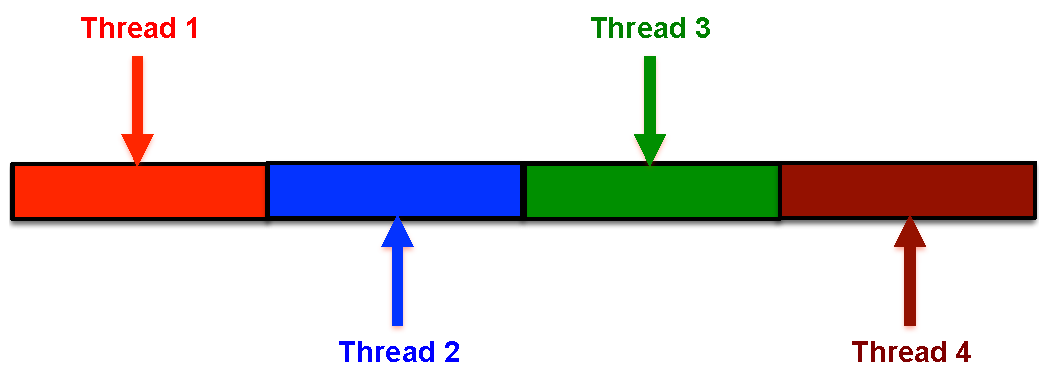
\includegraphics[width=2.4in]{sheriff/figure/falsesharing.pdf}
}%
\hspace{50pt}
\subfigure[True sharing]{%
   \label{fig:ts}
   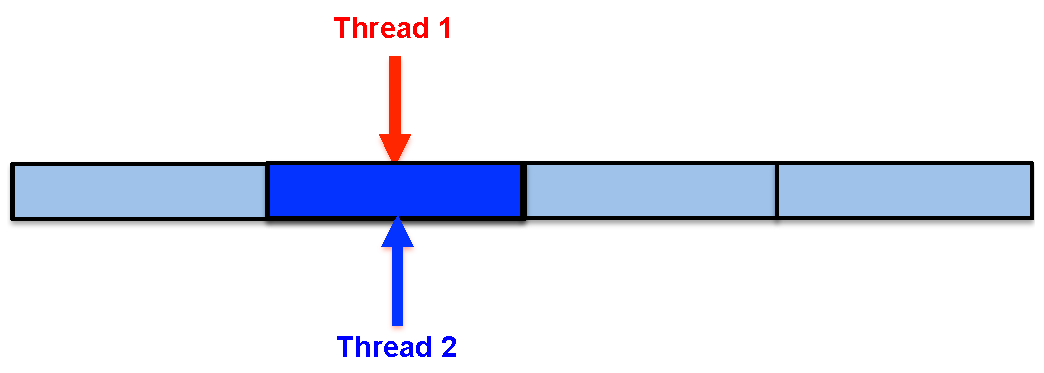
\includegraphics[width=2.4in]{sheriff/figure/truesharing.pdf}
}%
\end{center}
%\includegraphics{fig/potential.pdf}
\caption{False sharing and true sharing in a cache line with four words. }
\label{fig:fsexample}
\end{figure*}

% The classification of false sharing?

\subsection{Reason of False Sharing}

As shown in Figure~\ref{fig:fsexample}, false sharing only occurs when the size of coherence block is larger than that of a single word. Multiple processors may reference different words of the same coherence block. In this perspective, a single-word block size can avoid false sharing problems. 

However, using a single-word block size is not the actual case. In reality, the size of a coherence block (cache line) is normally 32 or 64 bytes. The reason of using multiple words in a cache line is to reduce the groups of transfers between the main memory and the cache since programs always have some spatial locality of reference. Those adjacent words are very likely to be referenced in the future.

From the performance perspective, reducing the coherence block size to one word may minimize the data to transferred, but can increase the number of transfers. Thus, the overhead of transferring less data at a time can be larger than the benefit of eliminating false sharing coherence traffic. Actually, the hardware trend of cache line is to increase the size of cache line, which makes false sharing problems increasingly common. 

\subsection{Performance Impact}
\label{falsesharing}
False sharing can greatly slowdown the execution of multithreaded programs, which depends on many factors, including the cache block size, data layout, program access patterns, and the cost of coherence operations~\cite{Bolosky:1993:FSE:1295480.1295483}. 

In a typical shared-memory system, each processor may have a separate cache. In order to increase the access speed, when a processor references a word, all the data inside the same cache line is fetched from the main memory to its corresponding cache. 
When multiple processors are accessing distinct words of the same cache line simultaneously, the shared data can be replicated into caches of different processors that access this cache line. Thus, it is very important to maintain the coherence across different processors: if any copy is changed, this change should be propagated to other processors immediately for correctness purposes. In real hardware, this data propagation only happens lazily when the data is accessed again, thus duplicates are invalidated at first. When a processor access an invalidated cache line, it should wait for the data propagating from other processors, wasting CPU time and memory bandwidth simultaneously. 

In the false sharing case, this propagation is totally unnecessary because different threads are actually accessing different parts of the same cache line. Thus, there is no need for a processor to get the updated data that is not going to access. However, hardware can only tracks the change of data on the granularity of a cache line and have to propagate those changes if any word has been changed. When there are interleaved writes, issued by different processors, on the same cache line, the ping-pong effect of loading-and-invalidating of data on this cache line can greatly slow the execution of programs. 
Programs with false sharing can even run slower in a multi-core machine than in a single-core machine, losing the benefit of multiple cores.  

Many common programming practices can easily cause false sharing. For example, different threads accessing different entries of the same global array, listed in Figure~\ref{fig:falsesharingexample}, is such an example. This example has no correctness problem, but a serious performance problem. 

\begin{figure*}[!ht]
{\centering
\fbox{
\subfigure{\lstinputlisting[numbers=none,frame=none,boxpos=t]{fig/falsesharing.sample1}}
\hspace{20pt}
\subfigure{\lstinputlisting[numbers=none,frame=none,boxpos=t]{fig/falsesharing.sample2}}
}
\caption{False sharing problem
\label{fig:falsesharingexample}}
}
\end{figure*}

We actually run this program on a real machine with 8 cores and Figure~\ref{fig:fsperfimpact} presents performance results. On this evaluation, we specifically choose a different number of threads, matching the number of hardware cores, from 1 thread to 8 threads, to perform the same amount of workload. We find out that false sharing can greatly impact the performance, which brings around $13\times$ difference between actual performance and the expected performance. Two trends--the prevalence of multicore architectures and
the expected increase in the number of multithreaded applications in broad use, and increasing cache line sizes--are likely to make false sharing increasingly common.

\begin{figure*}[!t]
\centering
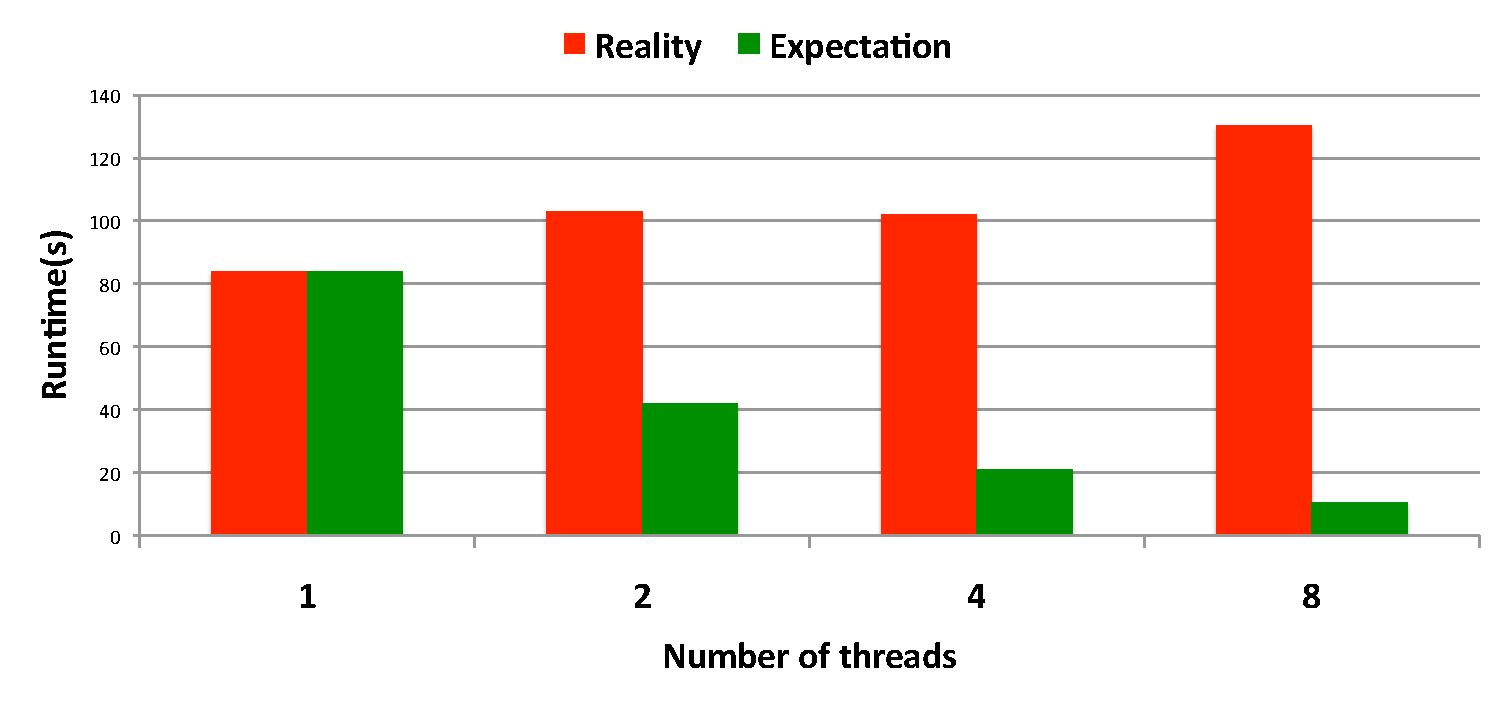
\includegraphics[width=5in]{fig/fsperfimpact.pdf}
\caption{
False sharing performance impact for the simple program shown in Figure~\ref{fig:falsesharingexample}.
\label{fig:fsperfimpact}
}
\end{figure*}

\subsection{Fixing False Sharing}
There are several ways to fix false sharing problems after they are identified. The basic idea is to prevent multiple threads from accessing the same cache line simultaneously.  

The first way is to change the size of corresponding structure or class, by padding some useless words. Thus, we can prevent two threads concurrently accessing the same cache line. One example of prevention, linear\_regression, can be seen in Section~\ref{sec:effecteval}.

The second way is to assign the value to thread-local variables at first. Then different threads only update their own local variables, and commit those changes back to the shared variable in the end. For example, the problem shown in Figure~\ref{fig:falsesharingexample} is fixed using this method, see Figure~\ref{fig:falsesharingexamplefix}. 

\begin{figure*}[!ht]
{\centering
\fbox{
\subfigure{\lstinputlisting[numbers=none,frame=none,boxpos=t]{fig/falsesharing.sample2fix}}
}
\caption{Fixing the false sharing problem shown in Figure~\ref{fig:falsesharingexample}.
\label{fig:falsesharingexamplefix}}
}
\end{figure*}

Some other approaches, to fix false sharing problems automatically, is described in detail in Section~\ref{sec:fspreventwork}, but they all suffer different shortcomings. 




